\documentclass[a4paper, 12pt]{article}
\usepackage[a4paper,textwidth=170mm,textheight=245mm]{geometry}

\usepackage[utf8]{inputenc}
\usepackage{todonotes}
\usepackage{amsmath}
\usepackage{parskip}
\usepackage{listings}
\usepackage{float}
\usepackage{url}
\usepackage{hyperref}

% For the wrapfigure
\usepackage{wrapfig}
\usepackage{caption}
\usepackage{subcaption}
\usepackage{color, colortbl}

\definecolor{Green}{rgb}{0.3,0.85,0.24}

\begin{document}
\date{March 2020}

\title{\Large SentimentalCrypto: Classification of Sentiment of the Cryptocurrency market and Clustering analysis}

\author{
{Omkar Bhutra}\\
{LIU ID: omkbh878}\\
{Course code: 732A92}\\
Statistics and Machine Learning
}

\maketitle

\newpage

\subsection*{Abstract}

Most Cryptocurrencies use Blockchain technology to record and distribute ledgers of transactions. The largest by market capitalisation are Bitcoin and Ethereum.

There exist over \textit{5000} cryptocurrencies, most of which are widely speculated and traded over a large number of exchanges online. This project aims to build a sentiment classification tool to establish the current sentiment of the cryptocurrency market based on twitter feed. Further, Clustering analysis is performed to better understand the twitter corpus 

\textit{320K} tweets that were segmented by emotions: \textit{anger, fear, greed, hateful, joy, sadness} were used to train our classifiers after preprocessing and classification training was done using Multinomial Naive Bayes, Logistic Regression, Stochastic Gradient Classifier and method with highest accuracy were chosen for further use. Valence Aware Dictionary and sEntiment Reasoner (VADER) was used to generate a polarity score and clustering analysis was performed on twitter corpus using K-Nearest Neighbors.

Finally, the chosen classifier was applied on completely unseen data pulled from Twitter using the Tweepy API to classify market sentiment as on \textit{7th March 2020}. Our classifier showed that the market was largely filled with 'Greed' and 'Fear' with a small propotion of 'Hateful. On 15th March 2020, 'fear' had increased and mixed emotions of 'sadness' and 'joy' were also present.

This project of classification of the current market sentiment was performed during the marketwide sell-off with drop in Bitcoin's price from 9000\$ to 4000\$ amidst the n-covid 19' pandemic where even global stock markets experienced major declines in sentiment.

\section{Introduction}
A Blockchain is a growing list of records called \textit{blocks} that are linked using concepts of cryptography. Such a list is distributed to all users participating in the network and thereby establishing decentralised trust. \cite{nakamotobitcoin}
As everything else in our world we order things and place them in different categories. Bitcoin is the first cryptocurrency that was invented in 2009 by a person who went by the pseudonym 'Satoshi Nakamoto' on Reddit. After the successful launch of the network and with enough network participants.

The task was to build a system for classification of current market sentiment of the cryptocurrencies. The topic of research was to observe what kind of classification models work best for such a corpus. The aim of the study was that this system should be able to aid trader's or investor's in making informed decisions.

After cryptocurrencies such as Bitcoin and Ethereum caught mainstream attention in 2017 and speculation on both its value and technology increased greatly , using a tool to monitor the sentiment of the cryptocurrency market can prove useful in making better investment decisions. Twitter is widely used platform where notable investors and developers of blockchain projects present their work and idea's. Tweeter can sometime's trigger market movements since they are often the first indications of press releases or announcements. Further, Clustering analysis was performed on the corpus of tweets to better understand our dataset and observe if there exists any explainable clusters with common knowledge of the blockchain space.

\pagebreak
\section{Theory}

\subsection{VADER Sentiment Intensity Analysis}
Valence Aware Dictionary and sEntiment Reasonor is a lexicon and rule-based sentiment analysis tool that is specifically tuned to sentiment in online social media text. It is sensitive to both polarity (positive/negative) and intensity (strength) of emotion. All lexical features of existing well-established and human validated sentiment lexicons along with additional lexical features that is used to express sentiment in social media text (emoticons,acronyms,slang) is used. A wisdom-of-the-crowd approach to establish point estimations of sentiment valance for each of the 9000+ lexical feature candidates and then keeps 7500+ lexical featires with mean valance close to 0 and standard deviation less than 2.5 as a human validated gold standard lexicon. Generalizable heuristics of the assessing sentiment in text is identified iteratively and point estimates of sentiment valance on the corpora from seperate domains.  \cite{gilbert2014vader}

\textit{VADER has been found to be quite successful when dealing with social media texts, NY Times editorials, movie reviews, and product reviews} \cite{pandey_vader_tutorial}

The valence score of a sentence is calculated by summing up the valence scores of each VADER-dictionary-listed word in the sentence. Cautious readers would probably notice that there is a contradiction: individual words have a valence score between -4 to 4, but the returned valence score of a sentence is between -1 to 1.

They’re both true. The valence score of a sentence is the sum of the valence score of each sentiment-bearing word. However, we apply a normalization to the total to map it to a value between -1 to 1. \cite{hutto_vader}

The normalisation rule is:
where x is the sum of valance scores and alpha is the normalization parameter that is set to a constant.
\large \dfrac{x}{\sqrt{x^2 + \alpha}}

\subsection{Naive Bayes}

Multinomial Naive Bayes build a probabilistic model that uses arbitrary features from documents. When training the model features are extracted from different documents and are given to the model together with the class labels.
For each feature and class the probability in formula \ref{eq:feat} is calculated where $ feat_{i}$ is feature i and $ class_k $ is class k.

\large
\begin{equation}
    p (feat_{i}|class_{k})
    \label{eq:feat}
\end{equation}
\normalsize

When predicting the class of a document the same features are extracted and given to formula \ref{eq:bayes} where there exist $K$ classes and $n$ features for each document.
The probability of the class is multiplied by all features explained in formula \ref{eq:feat}.
The predicted class k is the k that maximizes the expression.

\large
\begin{equation}
    \hat{y} = \underset{k \in \{1,2,...,K\}}{argmax} \, \, \, p(class_{k}) \prod_{i=1}^{n} p (feat_{i}|class_{k}
    \label{eq:bayes}
\end{equation}
\normalsize

The strength of the Naive Bayes classifier is that the features are arbitrary.
The model determine the importance for all features and let informative features influence the prediction as well as assign uninformative features with low probabilities. \cite{TextMininglecture} \cite{rish2001empirical}

\subsection{Logistic Regression}

Logistic regression (LR) is useful in many areas such as document classification and
natural language processing (NLP). It models the conditional probability as:

\large
\begin{equation}
    Pw(y = ±1|x) = 1/1 + e^−{ywTx}
    \label{eq:cond1}
\end{equation}
\normalsize

where x is the data, y is the class label, and w  R nis the weight vector. Given two-class training data {(xi, yi)}^{l}_{i=1}, xi \in \mathbb{R}^{n}, yi \in {1, −1}

\newline
Logistic regression minimizes the following regularized negative log-likelihood:
\large
\begin{equation}
P^{LR}(w) = C\sum^{l}_{i=1}log(1+e^{-y_{i}w^{T}x_{i}}) + \frac{1}{2}w^{T}w
    \label{eq:cond2}
\end{equation}
\normalsize

\cite{journals/ml/YuHL11}

\subsection{Stochastic Gradient Descent}

This estimator implements regularized linear models with stochastic gradient descent (SGD) learning: the gradient of the loss is estimated each sample at a time and the model is updated along the way with a decreasing strength schedule (learning rate). SGD allows minibatch (online/out-of-core) learning.
For best results using the default learning rate schedule, the data should have zero mean and unit variance. \cite{conf/kdd/ZadroznyE02}

This implementation works with data represented as dense or sparse arrays of floating point values for the features. The model it fits can be controlled with the loss parameter; by default, it fits a linear support vector machine (SVM).
\cite{journals/jmlr/ZhangDJ02}

\subsection{Classification report - Accuracy, precision , recall , f1-score and support}

Precision and recall ‘zoom in’ on how good a system is at
identifying documents of a specific class 𝑐.
Equations \ref{eq:prec} and \ref{eq:recall} are with respect to the positive class.

\begin{itemize}
    \item {\textbf{Precision} - Precision is the proportion of correctly classified documents
among all documents for which the system predicts class 𝑐.
				\begin{equation}
						Precision = \frac{no. of True positives}{no. True positives+no. False positives}
				\label{eq:prec}
				\end{equation}
						When the system predicts class 𝑐, how often is it correct?}
    \item {\textbf{Recall} - Recall is the proportion of correctly classified documents among
all documents with gold-standard class 𝑐.
				\begin{equation}
						Recall = \frac{no. of True positives}{no. True positives+no. False positives}
				\label{eq:recall}
				\end{equation}
When the document has class 𝑐, how often does the system predict it?}
    \item {\textbf{F1-measure} - A good classifier should balance between precision and recall. The F1-measure is the harmonic mean of the two values:
		
						\begin{equation}
						Recall = \frac{2. precisioon . recall}{precision + recall}
				\label{eq:f1}
				\end{equation}
			}
\end{itemize}
\cite{TextMininglecture}

\subsection{Clustering - k-Means}

\begin{itemize}
    \item {\textbf{k-means} - The k-means algorithm aims to partition a document collection
into 𝑘 clusters, minimising within-cluster variance in distance.
distance variance = squared Euclidean distances. Each document, represented by its vector, will be put into the
cluster with the nearest centroid (mean).}
    \item {\textbf{Centroids and medoids} - The centroid of a cluster is the arithmetic mean of the document
vectors in the cluster, not necessarily the vector of an actual document. The medoid of a cluster is a vector in the cluster whose average
distance to all the other vectors is minimal, not the same as a geometric median }
\end{itemize}

Issues with the k-means algorithm:
- The k-means algorithm always converges, but there is no guarantee that it finds a global optimum. Solution: random restarts
- The number of clusters needs to be specified in advance, or chosen based on heuristics and cross-validation. Example: elbow method
- The k-means algorithm is not good at handling outliers – every document will eventually belong to some cluster.
\cite{TextMininglecture}

\section{Data}
\label{sec:dataset}

\subsection{Emotions in Cryptocurrency related tweets}
The following criterions were considered when looking for a corpus of tweets:
\begin{itemize}
    \item {\textbf{Class labels} - Data tagged with a gold standard class label tagged by humans .}
    \item {\textbf{Reliable} - The compiler behind the dataset should have good score on kaggle.}
    \item {\textbf{Large corpus} - Covers tweets from a large timeframe to include tweets from varied market conditions, atleast 2 years}
    }
    \item {\textbf{Volume of data} - To achieve a reliable classification we must have atleast a few hundred thousand tweets.}
\end{itemize}

\subsection{Training and Testing Twitter data}
The datasets for each of the 6 emotions are taken and merged. \cite{twitterdata_Zolkepli} 
"#bitcoin" and "#crypto" are the filters used to make 6 datasets by the author, \textit{anger}, \textit{greed}, \textit{fear}, \textit{hateful}, \textit{joy} and \textit{sadness} are the emotions that are used as class labels.
This data is merged and and a column for class labels is created which are gold standard class labels as they are human verified sentiments in tweets related to the cryptocurrency market. The data is preprocessed and cleaned by the same process as for the training and testing dataset. see \ref{sec:Method} for steps in preprocessing.


Table \ref{tab:cleanedtext} shows a subset of the preprocessed string of textual data from the tweets which is used by the classification models.
\begin{table}[h]
\begin{center}
    \begin{tabular}{| r | l | r |}
        \hline
        id  				& Preprocessed text    												&emotion		\\ \hline
        100001       & digitalvillain tech company still care ai iot ...     & greed \\ \hline
        100002       & commenters saying could pay lower fee wait mis... 	 & greed\\ \hline
        100003       & senior research scientist robotics startup cyb...     & greed \\ \hline
        100004       & current top dapps volumelastday kyber idex for...   & greed  \\ \hline
        100005       & cinsbit pleased announce fortem capital token ...   & greed   \\ \hline
				...     & ...																										& ...	\\ \hline
        328358       & zackvoell digital gold every function gold bet...   & sadness    \\ \hline
        328359       & never see adoption principle privacy fungibili...   & sadness  \\ \hline
        328360       & blockbits incent target broken economy reward ...    & sadness   \\ \hline
        328361       & sad cant proud watching world getting decentra...     & sadness    \\ \hline
        328362       & sad thing sheep buy po												      & sadness\\ \hline
    \end{tabular}
    \caption{Preprocessed string from the tweets }
    \label{tab:cleanedtext}
\end{center}
\end{table}


Figure \ref{fig:tweetsdata} shows the number of tweets by all emotions. This dataset is used for training and testing of the model after randomized shuffling and a split with a ratio of 70/30 for training vs test data.
In figure \ref{fig:tweetsdata}\textit{a} shows the training and test split \ref{fig:tweetsdata}\textit{b} shows the undersampled data vs the training data , by emotion.
\begin{figure}[H]
    \centering
    \begin{subfigure}[b]{0.48\textwidth}
        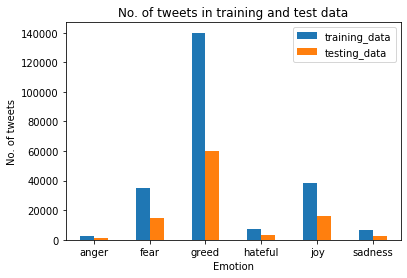
\includegraphics[width=\textwidth]{res/training_test.png}
        \caption{Number of tweets in training and test data}
    \end{subfigure}
    ~ % spacing
    \begin{subfigure}[b]{0.48\textwidth}
        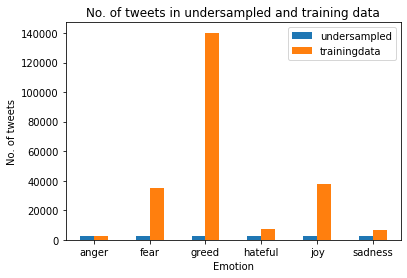
\includegraphics[width=\textwidth]{res/undersampled_training.png}
        \caption{Number of tweets in undersampled and training data}
    \end{subfigure}
    \caption{Histograms of number of tweets by emotions}
    \label{fig:tweetsdata}
\end{figure}

\subsection{Current Twitter data}
Tweepy is used along with the developer's API for twitter to bring current data to classify using our model for the purpose of use in trading and investing.  \cite{tweepy} cite{\bs4}

Future work with this dataset can include this data into the testing of the classifier after labelling this datasest with an emotion class manually. \ref{sec:Conclusion}

Using the API a search query "#bitcoin" and "#crypto" is sent with the current date, Retweets are filtered to avoid duplicates in out corpus. The data is compiled by user,location and the tweet text. The data is preprocessed and cleaned by the same process as for the training and testing dataset. see \ref{sec:Method} for steps in preprocessing.

Figure \ref{fig:currenttweetsdata} shows current stream of tweets tagged by \textit{'#bitcoin'} or \textit{'#crypto'}
\begin{figure}[H]
    \centering
    \begin{subfigure}[b]{0.8\textwidth}
        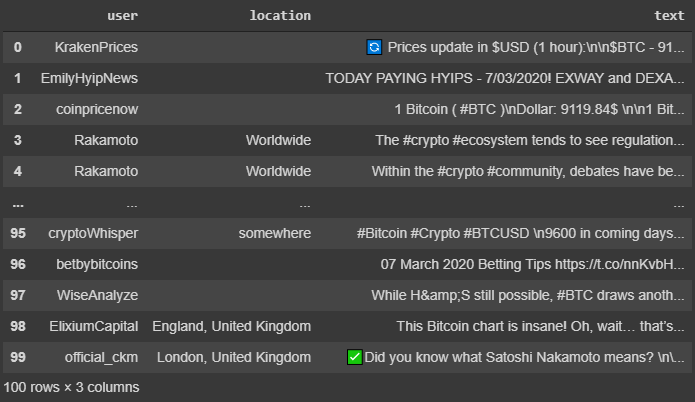
\includegraphics[width=\textwidth]{res/currenttweets1.png}
    \end{subfigure}
    \caption{Table of current tweets with no class labels, by user , location and text in the tweets}
    \label{fig:currenttweetsdata}
\end{figure}


\subsection{Code}
The complete code for this project can be found at GitHub. \cite{github}
Documentation on how to retrieve the corpus and run the system can be found in the repository.
Future work and updates on this project can be found on the same github repository.

\pagebreak
\section{Method}
\label{sec:Method}
\begin{itemize}
    \item {\textbf{Dataset} - Tweets were segmented by emotions like \textit{anger}, \textit{fear} ,\textit{greed} ,\textit{hateful}, \textit{joy} and \textit{sadness}. This data was taken from Kaggle and it consisted around 320,000 tweets in separate datasets for each emotion and it is an unbalanced raw dataset of tweets from which class labels for emotions are generated into a single large dataset. \cite{twitterdata_Zolkepli} \cite{mydataomkar}}
    \item {\textbf{Data preprocessing} - The tweets were preprocessed in the following order: punctuation removal, link/url removal and tokenization using the library 're', stopword removal and removal of some specific words that to reduce noise using the package 'nltk' \cite{nltk} , Stemming / Lemmatisation. \cite{inproceedings} \cite{pandey_vader_tutorial}. Wordclouds of the cleaned string of words are produced for each 'emotion' class.}
    \item {\textbf{Sentiment Intensity} - The VADER algorithm was applied only on the punctuation cleaned tweets and this gives the a polarity index between -1 and 1 for each tweet. -1 representing extreme negative sentiment and +1 representing extreme positive sentiment. This is visualised by a violin plot of the polarity score on the y-axis, named 'compound'  the dataset Vs the 6 'emotion' classes on the x-axis. The library 'vaderSentiment' is used and the 'SentimentIntensityAnalyzer' class is initialized and only the punctiation removed tweets\cite{gilbert2014vader}}
		\item {\textbf{Training and Testing data} - The corpus of tweets in the training and test data consisted each tweet is has a class label one of 6 'emotion' types.The corpus was shuffled after importation.The seed for the random state function is initialized with a constant value of 42 to ensure reproducibility.
    \item {\textbf{Classification} - Multinomial Naive Bayes, Logistic Regression and Stochastic Gradient Descent Classifier are used  duting thethe modelling process. The method which produces the highest accuracy is chosen for further predictions.}
		\item {\textbf{Prediction of the classifier on current tweets} - 500 Current tweets are streamed through the \textit{tweepy API}, Preprocessed in the same way as the training and test dataset, VADER sentiment is calculated and prediction of the class label is done using the classifier with the highest accuracy.
}
\end{itemize}

\subsection{Wordclouds}
\label{sec:Wordclouds}
Wordclouds are generated for the purpose of visualisation of the preprocessed tweets that are used in the classifiers.
The wordclouds for all emotions as well as by each emotion are produced using the library \textit{wordcloud} using the functions \textit{WordCloud}, \textit{'ImagColorGenerator'}. 

\begin{itemize}
    \item {\textbf{Maximum words} -  100}
    \item {\textbf{Interpolation} -  bilinear}
}
\end{itemize}

\subsection{Sentiment Intensity}
\label{sec:sentimentintensity}
Punctuations are removed from all the tweets  and this data is used in the VADER Sentiment Intensity analyser.

Table \ref{tab:punctext} shows a subset of the only the punctuation removed text from tweets which is used by the VADER sentiment intensity analyser.
\begin{table}[h]
\begin{center}
    \begin{tabular}{| r | l | r |}
        \hline
        id  				& Punctuation removed text    												&emotion		\\ \hline
        100001       & DigitalVillain Tech companies still care mo...      & greed \\ \hline
        100002       & All the commenters saying he could pay a lower... 	 & greed\\ \hline
        100003       & Senior Research Scientist Robotics Startup C...     & greed \\ \hline
        100004       & current top dapps volumelastday kyber idex for...   & greed  \\ \hline
        100005       & cinsbit pleased announce fortem capital token ...   & greed   \\ \hline
				...     & ...																										& ...	\\ \hline
        328358       & zackvoell Bitcoin is digital gold it does ever...   & sadness    \\ \hline
        328359       & Bitcoin BTC will never see adoption if princip...   & sadness  \\ \hline
        328360       & BlockBits Incent Targets Broken Economy With B...    & sadness   \\ \hline
        328361       & So sad that I cant be there but so proud to be...     & sadness    \\ \hline
        328362      & Sad thing is sheep will buy into this POS 	...      & sadness\\ \hline
    \end{tabular}
    \caption{Punctuation cleaned from the tweets }
    \label{tab:punctext}
\end{center}
\end{table}

The polarity scores vs emotion type for all the tweets are visualised in a violin plot. This includes summary statistics of the data, the box plot, interquartile ranges, density plot.


\subsection{Baseline}
\label{sec:baseline}
The classifier was initialized with the randomly shuffled corpus and the data was split up into training data and test data.
The default values were $70\%$ training data and $30\%$ test data
The baseline accuracy is calculated as the average number of cases where the mode of emotion types of the training data are equal to the emotion types in the test data. 

\subsection{Classification}
\label{sec:Classification}

Multinomial Naive Bayes, Logistic Regression and Stochastic Gradient Descent Classifier are used  during the modelling process. The method which produces the highest accuracy is chosen for further use in the study.

\begin{itemize}
	  \item {\textbf{Naive Bayes} - Multinomial Naive Bayes is applied on the training data in a pipeline with \textit{CountVectorizer} and \textit{MultinomialNB} functions from the \textit{sklearn} library , the overall accuracy,classification report an the confusion matrix are produced.
Undersampling without replacement is performed based on the a random choice function from the \textit{numpy} library and a balanced dataset is produced to calculate the undersampled accuracy of the Naive Bayes model.
GridSearch Cross Validation is performed on the Naive Bayes model to see if the results are consistent.
Other summary statistics such as precision, recall, f1-score and support are also shown in the classification reports.

		\item {\textbf{Logistic Regression} - Logistic Regression is applied on the training data in a pipeline with \textit{CountVectorizer} and \textit{LogisticRegression} functions from the \textit{sklearn} library , the overall accuracy, classification report an the confusion matrix are produced.
}

\item {\textbf{Stochastic Gradient Descent} - \textit{SGDClassifier} is applied on the training data in a pipeline with \textit{CountVectorizer} and \textit{LogisticRegression} functions from the \textit{sklearn} library, lbfgs optimality is used \cite{journals/ml/YuHL11} .The overall accuracy, classification report an the confusion matrix are produced. Grid Search Cross Validation is performed for the logistic regression model
}

\end{itemize}

\subsection{Clustering - k-means}

Hard clustering is done using k-means from the \textit{sklearn} library. They elbow point is analysed upto k = 10 iteratively. 
The elbow method lead us to check for k = 2 and 8.

We can compute rand indices since we have gold standard class labels. The rand index and adjusted rand score is calculated for both the chosen k cases. 5 terms with highest centroid values are identified for each cluster in both the cases.


\section{Results}
The results will focus mainly on comparing two different genres or comparing all genres.
For all tests the split in training and test is 70\% and 30\% respectively.
Cross validation is 5-fold.
All other arguments use the default values.
Between different tests the random seed was reset which makes the results reproducible.

Performance for the baseline system is shown in table \ref{tab:cr1}.

\subsection{Baseline}
Classification report for the model is given in the table \ref{tab:cr1}.
A baseline accuracy of 60.83\% is achieved.

\begin{table}[h]
\begin{center}
    \begin{tabular}{| r | r | r | r | r | }
        \hline
      emotion & precision & recall & f1-score & support \\ \hline
      anger    & 0.12  & 0.93     & 0.21   		& 1097    \\ \hline
			fear		& 0.78     & 0.72     & 0.75   & 15038 \\ \hline
      greed    & 0.96     & 0.56     & 0.71   & 59928 \\ \hline
      hateful    & 0.35     & 0.76     & 0.48   & 3139 \\ \hline
      joy       & 0.72   &0.86     & 0.78    & 16401 \\ \hline
      sadness    & 0.18    & 0.93     & 0.31  & 2906  \\ \hline
									 &      &        &           &     \\ \hline
      accuracy     &   			&   		 		& 0.66  &98509    \\ \hline
      macro avg     & 0.52   &0.79        & 0.54  &98509   \\ \hline
		  weighted avg & 0.84   &0.66       & 0.70   &98509  \\ \hline
    \end{tabular}
    \caption{Classification report of the Naive Bayes model}
    \label{tab:cr1}
\end{center}
\end{table}

The Confusion Matrix is given in the figure \ref{fig:con1}
\textit{greed} has the highest number of true positives, followed by \textit{joy} and \textit{fear}
 
\begin{figure}[H]
    \centering
    \begin{subfigure}[a]{0.48\textwidth}
        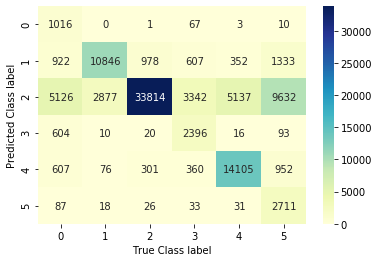
\includegraphics[width=\textwidth]{res/con1.png}
        \caption{Confusion Matrix for the Balanced dataset}
    \end{subfigure}
		\caption{Confusion Matrix}
		\label{fig:con1}
\end{figure}


\subsection{Most common words by emotion}
\label{sec:wordclouds1}

Figure \ref{fig:wordcloud_angreed} in \textit{a-e} shows the show most common words by emotion \textit{anger,fear,greed,hateful,joy and sadness}
\begin{figure}[H]
    \centering
    \begin{subfigure}[a]{0.3\textwidth}
        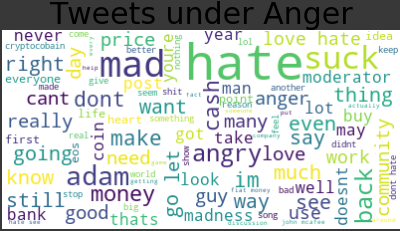
\includegraphics[width=\textwidth]{res/wordcloud_anger.png}
        \caption{Common words in the twitter corpus by anger}
    \end{subfigure}
    ~ % spacing
    \begin{subfigure}[b]{0.3\textwidth}
        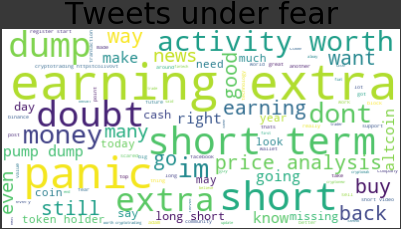
\includegraphics[width=\textwidth]{res/wordcloud_fear.png}
        \caption{Common words in the twitter corpus by fear}
    \end{subfigure}
		~ % spacing
    \begin{subfigure}[c]{0.3\textwidth}
        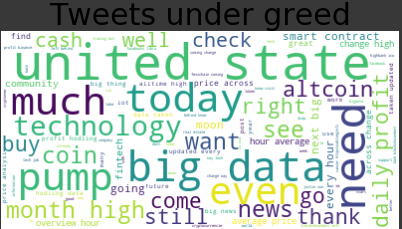
\includegraphics[width=\textwidth]{res/wordcloud_greed.png}
        \caption{Common words in the twitter corpus by greed}
    \end{subfigure}
		~ % spacing
    \begin{subfigure}[d]{0.3\textwidth}
        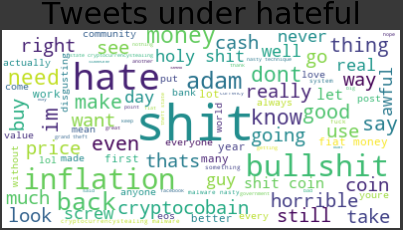
\includegraphics[width=\textwidth]{res/wordcloud_hateful.png}
        \caption{Common words in the twitter corpus by hateful}
    \end{subfigure}
    ~ % spacing
    \begin{subfigure}[e]{0.3\textwidth}
        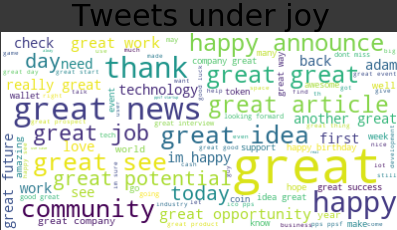
\includegraphics[width=\textwidth]{res/wordcloud_joy.png}
        \caption{Common words in the twitter corpus by joy}
    \end{subfigure}
		~ % spacing
    \begin{subfigure}[f]{0.3\textwidth}
        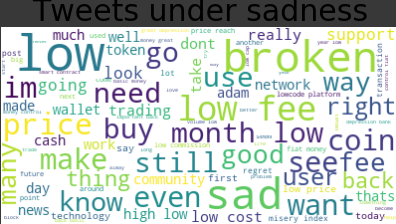
\includegraphics[width=\textwidth]{res/wordcloud_sadness.png}
        \caption{Common words in the twitter corpus by sadness}
    \end{subfigure}
		    \caption{Wordclouds from the tweets by emotion}
    \label{fig:wordcloud_angreed}				
\end{figure}


\subsection{VADER}
A sentiment intensity score is produced for each tweet based on only punctuation removed tweets without the use of class labels. \ref{sec:sentimentintensity}
\begin{figure}[H]
    \centering
    \begin{subfigure}[a]{0.99\textwidth}
        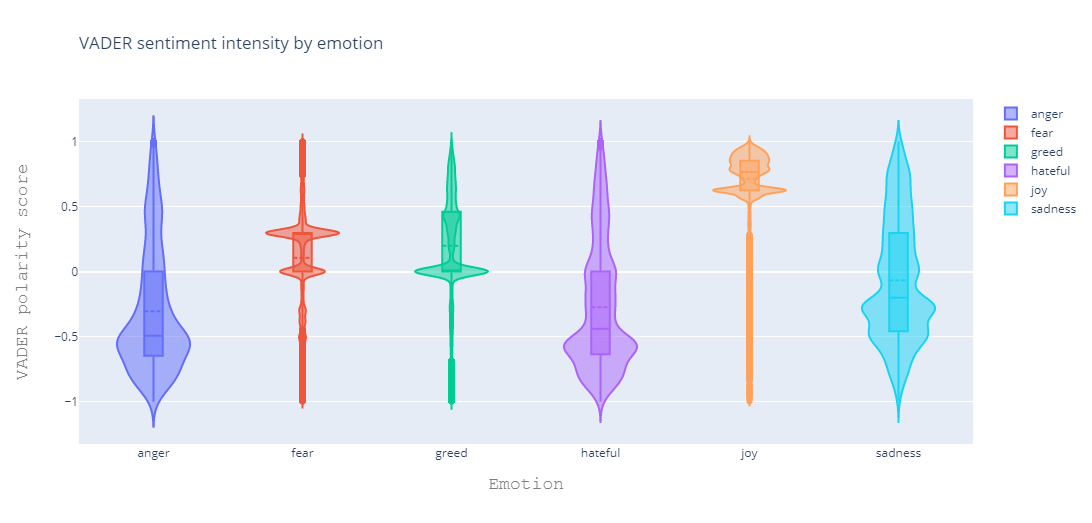
\includegraphics[width=\textwidth]{res/vaderinitial.png}
        \caption{VADER Sentiment Intensity vs Emotion}
    \end{subfigure}
		\caption{Violin Plot}
		\label{fig:violin}
\end{figure}

\begin{table}[H]
\begin{center}
    \begin{tabular}{| r | r | r | r | r | r | r |}
        \hline
        anger & fear & greed & hateful & joy & sadness & Summary \\ \hline
        -0.30 &  0.10 &  0.20 &  -0.27 &   	0.71	& -0.07 & mean \\ \hline
        -0.49  & 0.29 &  0 &  -0.44 &  0.765 &	-0.20		& median \\ \hline
        -0.55 & 0.29&   -0.003 &  -0.58 &   0.62 &  -0.29  & mode (density plot) \\ \hline
        -0.65 &  0 & 		0 &   			-0.63&   0.62 &  -0.45 & 1st Quantile (box plot) \\ \hline
         0 & 0.296 & 		0.45 &   				0 &   0.85 &  0.29 &  3rd Quantile (box plot) \\ \hline
    \end{tabular}
    \caption{Summary statistics from the violin plot}
    \label{tab:violintab}
\end{center}
\end{table}

This score is specifically designed to analyze the sentiment from social media text.
Summary stat are given in the table \ref{tab:violintab} and the plot is shown in figure \ref{fig:violin}

\subsection{Naive Bayes}
The classifier achieved an accuracy of 85.86\%. 5 fold Cross validation, which marginally improve the performance.

Classification report for the model is given in the table \ref{tab:cr2}.

\begin{table}[h]
\begin{center}
    \begin{tabular}{| r | r | r | r | r | }
        \hline
      emotion & precision & recall & f1-score & support \\ \hline
      anger    & 0.84  & 0.08     & 0.15   		& 1097    \\ \hline
			fear		& 0.85     & 0.71     & 0.81   & 15038 \\ \hline
      greed    & 0.85     & 0.96     & 0.90   & 59928 \\ \hline
      hateful    & 0.79     & 0.45     & 0.57   & 3139 \\ \hline
      joy       & 0.85   &0.86     & 0.86    & 16401 \\ \hline
      sadness    & 0.94   & 0.24     & 0.38  & 2906  \\ \hline
									 &      &        &           &     \\ \hline
      accuracy     &   			&   		 		& 0.86  &98509    \\ \hline
      macro avg     & 0.87   &0.55        & 0.61  &98509   \\ \hline
		  weighted avg & 0.86   &0.86       & 0.85   &98509  \\ \hline
    \end{tabular}
    \caption{Classification report of the Naive Bayes model}
    \label{tab:cr2}
\end{center}
\end{table}

The Confusion Matrix is given in the figure \ref{fig:con_nb}
\textit{greed} has the highest number of true positives, followed by \textit{joy} and \textit{fear}
 
\begin{figure}[H]
    \centering
    \begin{subfigure}[a]{0.48\textwidth}
        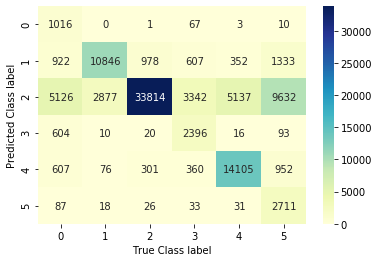
\includegraphics[width=\textwidth]{res/con1.png}
        \caption{Confusion Matrix for the Naive Bayes model}
    \end{subfigure}
		\caption{Confusion Matrix}
		\label{fig:con_nb}
\end{figure}


\subsection{Logistic Regression}
The accuracy of the model achieved is 94.36\%.

Classification report for the model is given in the table \ref{tab:cr3}.

\begin{table}[h]
\begin{center}
    \begin{tabular}{| r | r | r | r | r | }
        \hline
      emotion & precision & recall & f1-score & support \\ \hline
      anger    & 0.68  & 0.70     & 0.69   		& 1097    \\ \hline
			fear		& 0.93     & 0.89     & 0.91   & 15038 \\ \hline
      greed    & 0.96     & 0.96     & 0.96   & 59928 \\ \hline
      hateful    & 0.85     & 0.84     & 0.85   & 3139 \\ \hline
      joy       & 0.94   &0.96     & 0.95    & 16401 \\ \hline
      sadness    & 0.86    & 0.87     & 0.86  & 2906  \\ \hline
									 &      &        &           &     \\ \hline
      accuracy     &   			&   		 		& 0.94  &98509    \\ \hline
      macro avg     & 0.87   &0.87        & 0.87  &98509   \\ \hline
		  weighted avg & 0.94   &0.94       & 0.94   &98509  \\ \hline
    \end{tabular}
    \caption{Classification report of the Naive Bayes model}
    \label{tab:cr3}
\end{center}
\end{table}

The Confusion Matrix is given in the figure \ref{fig:con3}
\textit{greed} has the highest number of true positives, followed by \textit{joy} and \textit{fear}
 
\begin{figure}[H]
    \centering
    \begin{subfigure}[a]{0.48\textwidth}
        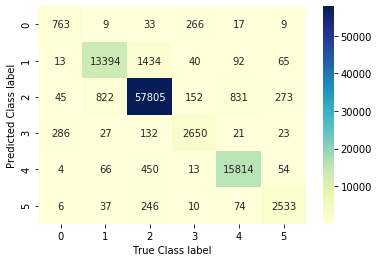
\includegraphics[width=\textwidth]{res/con_lr.png}
        \caption{Confusion Matrix for the Logistic Regression model}
    \end{subfigure}
		\caption{Confusion Matrix}
		\label{fig:con3}
\end{figure}

\subsection{Stochastic Gradient Descent}
The accuracy of the model achieved is 93.02\%.

Classification report for the model is given in the Table \ref{tab:cr4}.

\begin{table}[h]
\begin{center}
    \begin{tabular}{| r | r | r | r | r | }
        \hline
      emotion & precision & recall & f1-score & support \\ \hline
      anger    & 0.66  & 0.72     & 0.69   		& 1030    \\ \hline
			fear		& 0.94     & 0.81     & 0.87   & 15163 \\ \hline
      greed    & 0.95     & 0.96     & 0.95   & 60089 \\ \hline
      hateful    & 0.85     & 0.82     & 0.83   & 3072 \\ \hline
      joy       & 0.92  	&0.98     & 0.95    & 16298 \\ \hline
      sadness    & 0.82    & 0.87     & 0.84  & 2857  \\ \hline
									 &      &        &           &     \\ \hline
      accuracy     &   			&   		 		& 0.93  &98509    \\ \hline
      macro avg     & 0.86   &0.86        & 0.86  &98509   \\ \hline
		  weighted avg & 0.93   &0.93       & 0.93   &98509  \\ \hline
    \end{tabular}
    \caption{Classification report of the Naive Bayes model}
    \label{tab:cr4}
\end{center}
\end{table}

The Confusion Matrix is given in the Figure \ref{fig:con_sgd}
\textit{greed} has the highest number of true positives, followed by \textit{joy} and \textit{fear}
 
\begin{figure}[H]
    \centering
    \begin{subfigure}[a]{0.48\textwidth}
        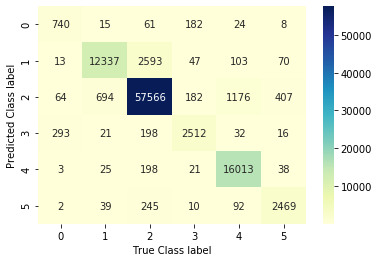
\includegraphics[width=\textwidth]{res/con_sgd.png}
        \caption{Confusion Matrix using Stochastic Gradient Descent}
    \end{subfigure}
		\caption{Confusion Matrix}
		\label{fig:con_sgd}
\end{figure}

5-fold cross validation allows for tuning of the model.
Best score: 0.929
Best parameters set: alpha =  1e - 05, max iterations = 20 ,penalty = 'elasticnet', tfidf idf use = False, vect.max.df = 0.5 ,n-gram range =  (1, 2)


\subsection{Prediction of current sentiment}
100 tweets filtered by the tags \textit{'Bitcoin'} and \textit{'Crypto'} are streamed using the api.  \ref{sec:Method}
Preprocessing is performed in the same way as training and test dataset. VADER sentiment is calculated and trained Logistic Regression classifier is used to classify the current emotion of the market.

\begin{figure}[H]
    \centering
    \begin{subfigure}[a]{0.99\textwidth}
        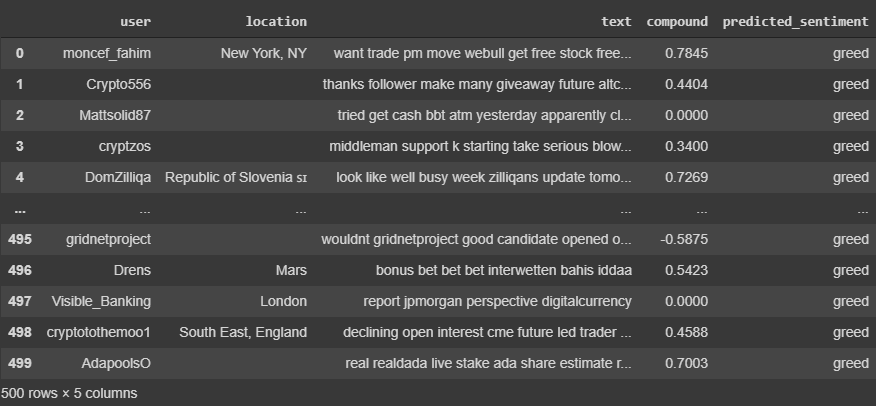
\includegraphics[width=\textwidth]{res/currenttweets_res.png}
        \caption{VADER sentiment intensity in current stream of tweets}
    \end{subfigure}
		\caption{Sentiment intensity}
		\label{fig:senint}
\end{figure}

\begin{figure}[H]
    \centering
    \begin{subfigure}[a]{0.99\textwidth}
        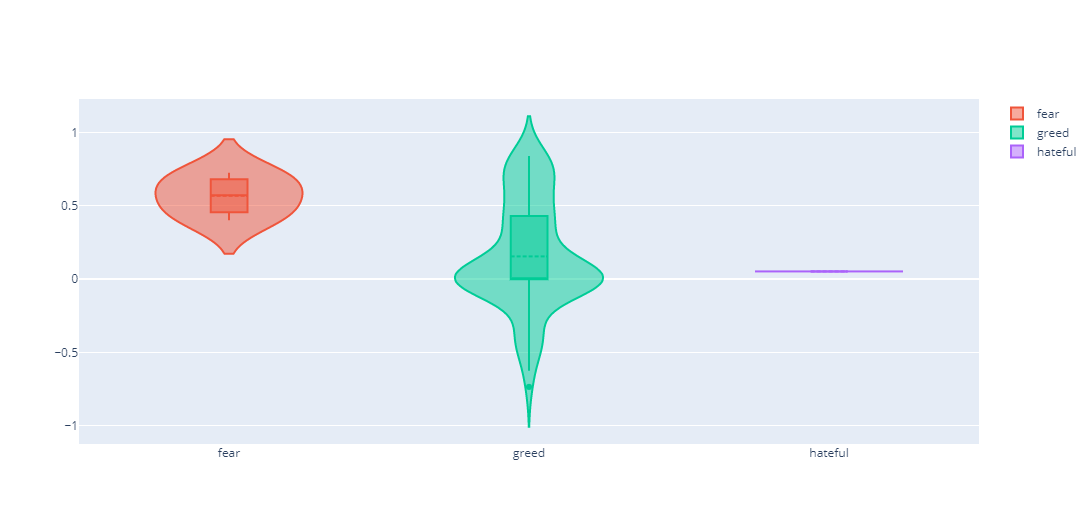
\includegraphics[width=\textwidth]{res/vaderfinal.png}
        \caption{VADER Sentiment Intensity vs Emotion - March 7, 2020}
    \end{subfigure}
		\caption{Violin plot}
		\label{fig:violin2}
\end{figure}

\begin{figure}[H]
    \centering
    \begin{subfigure}[a]{0.99\textwidth}
        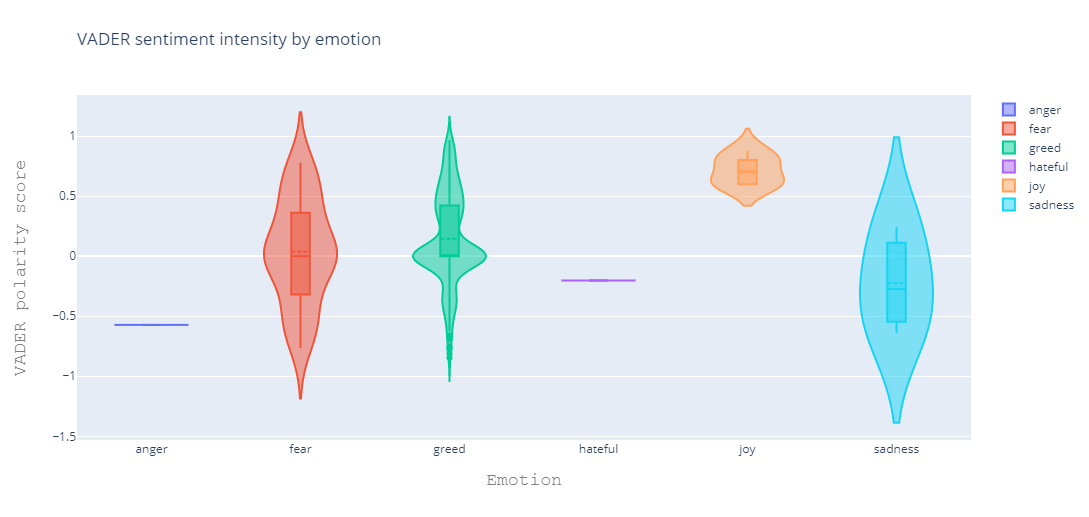
\includegraphics[width=\textwidth]{res/vaderfinalmarch15.png}
        \caption{VADER Sentiment Intensity vs Emotion - March 15, 2020}
    \end{subfigure}
		\caption{Violin plot}
		\label{fig:violin3}
\end{figure}


Summary stat are given in the table \ref{tab:violintab4} and the plot is shown in figure \ref{fig:violin3}

\begin{table}[H]
\begin{center}
    \begin{tabular}{| r | r | r | r | r | r | r |}
        \hline
        anger & fear & greed & hateful & joy & sadness & Summary \\ \hline
        -0.59 &  0.057 &  0.14 &  -0.2 &   	0.71	& -0.22 & mean \\ \hline
						-	& 0 		 &  0 &   &   -   &	-0.70		& -0.27    & median \\ \hline
						-	& 0.225  & -0.004 &   -   &   0.62   &  -0.31  & mode (density plot) \\ \hline
						-	& -0.32  & -0.005 &   -   &   0.60   &  -0.55 & 1st Quantile (box plot) \\ \hline
						-	& 0.40   &  0.42 &   	-	 &   0.802  &  0.11 &  3rd Quantile (box plot) \\ \hline
    \end{tabular}
    \caption{Summary statistics from the violin plot}
    \label{tab:violintab4}
\end{center}
\end{table}

\begin{table}[H]
\begin{center}
    \begin{tabular}{| r | r |}
        \hline
        predicted sentiment & count  \\ \hline
        anger   &  1  \\ \hline
				fear	  & 40 	\\ \hline
				greed	  & 451 \\ \hline
				hateful	& 1   \\ \hline
				joy			 & 5  \\ \hline
				sadness  & 2	\\ \hline
    \end{tabular}
    \caption{Count of predicted classes on current tweets}
    \label{tab:counter}
\end{center}
\end{table}

\subsection{Clustering - k-means}

\begin{figure}[H]
    \centering
    \begin{subfigure}[a]{0.9\textwidth}
        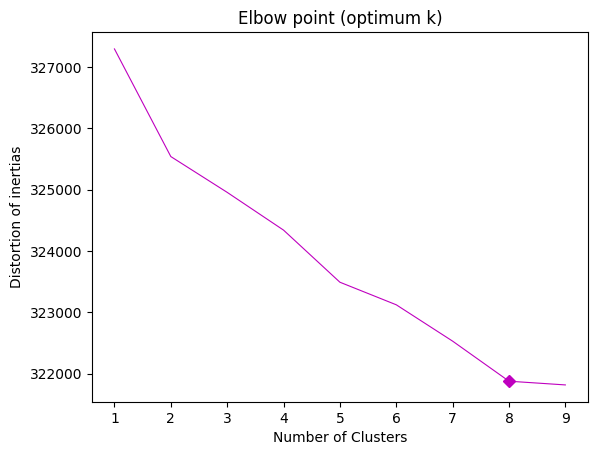
\includegraphics[width=\textwidth]{res/elbow.png}
        \caption{Elbow method to find optimum k}
    \end{subfigure}
		\caption{Elbow point}
		\label{fig:elbow}
\end{figure}


Three possible values for k can be chosen. 2,5 and 8. All are attempted but 8 provides with coherent terms in its clusters.


\begin{figure}[H]
    \centering
    \begin{subfigure}[a]{0.3\textwidth}
        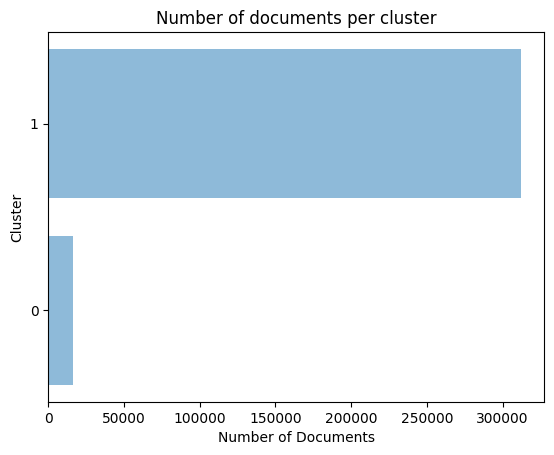
\includegraphics[width=\textwidth]{res/k2.png}
        \caption{Number of terms in clusters}
    \end{subfigure}
    ~ % spacing
    \begin{subfigure}[b]{0.3\textwidth}
        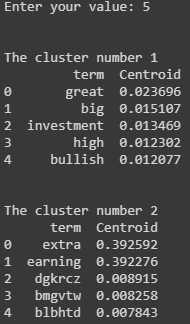
\includegraphics[width=\textwidth]{res/k2.1.png}
        \caption{Cluster terms with their centroids}
    \end{subfigure}
		\caption{ k = 2}
    \label{fig:k2}				
\end{figure}


\begin{figure}[H]
    \centering
    \begin{subfigure}[a]{0.6\textwidth}
        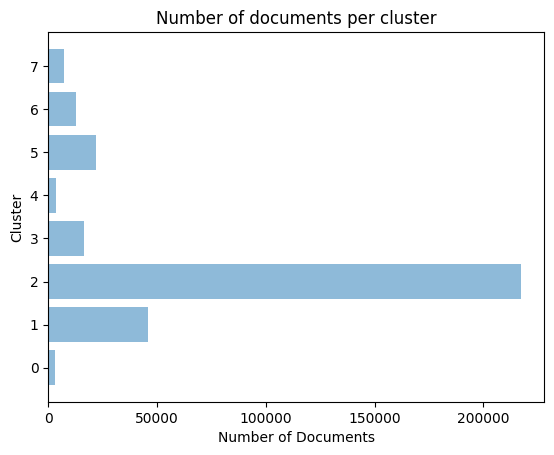
\includegraphics[width=\textwidth]{res/k8.png}
        \caption{Number of terms in clusters}
    \end{subfigure}
\end{figure}

\begin{figure}[H]
    \centering
    \begin{subfigure}[a]{0.3\textwidth}
        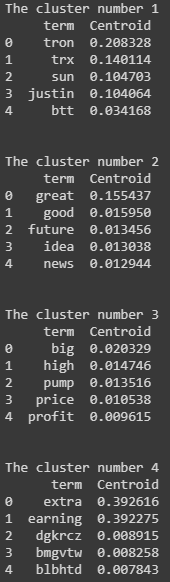
\includegraphics[width=\textwidth]{res/k8.1.png}
        \caption{Cluster terms with their centroids}
    \end{subfigure}
    ~ % spacing
    \begin{subfigure}[b]{0.3\textwidth}
        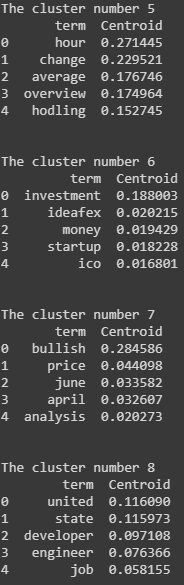
\includegraphics[width=\textwidth]{res/k8.2.png}
        \caption{Cluster terms with their centroids}
    \end{subfigure}
		\caption{ k = 8}
    \label{fig:k8}				
\end{figure}



\pagebreak
\section{Discussion}

Wordclouds by emotion typse provide us with a good first look into the data. tweets labelled with \textit{anger} have common words such as \textit{(hate,suck,mad,angry)},
with \textit{fear} have common words such as \textit{(short,panic,dump,doubt)} (In our data, 'short' would usually refer a short position that traders take when they bet on the price decreasing),
with \textit{greed} have common words such as \textit{(pump,big,high,buy)},
with \textit{hateful} have common words such as \textit{(hate,shit,bullshit,horrible)},
with \textit{joy} have common words such as \textit{(great,happy,thank,announcement)},
with \textit{sadness} have common words such as \textit{(low,sad,broken,sell)} 

The results of the baseline system are found in table \ref{tab:cr1}.
Using all emotions, the baseline system have the accuracy $60.83\%$. Undersampling resulted in a balanced dataset, when tested with the Naive Bayes classifier produced a 67.37\% accuracy.

The performance of Stochastic Gradient Descent was very close to that of Logistic Regression with 93.02\% accuracy with precision, recall and f1-score's only marginally lower.
The highest accuracy is achieved with the Logistic Regression Classifier of 94.26\% and hence that is used to classify the current market sentiment.
The lowest precision, recall and f1-score was produced for the class \textit{anger} and the highest for class \textit(greed). The bulk of the classified is emotion type \textit(greed).
The logistic regression method and the SGD classifier method are marginally different in their performance parameters , this can be seen in the confusion matrices in the figure \ref{fig:con_lr} and figure \ref{fig:con_sgd}.

The dataset is relatively unique and while comparing to results from other studies where VADER is used, it is noted that, other studies create \textit{silver standard} class labels as compared to the human tagged class labels in the dataset used in this study.
In the studies with the application of VADER , \cite{rochoz_cryptosentiment} Rochoz calculates the sentiment intensity by each cryptocurrency and studies how the index correlates with the price of that cryptocurrency. \cite{Thesken_altmonitor} J.Thesken uses the output of the sentiment index as inputs to a linear regression model. Similarly, In the paper by E.Linquist  \cite{kthbtcsentiment} the author has used bigrams, trigrams to identify suspicious bot tweets and remove them as part of preprocessing and performed used VADER sentiment to classify social media data related to cryptocurrencies in either positive, neutral or negative sentiment class.


It is observed in the figure \ref{fig:k8}	, the clustering with k = 8 provides a distinct coherent cluster's. The first cluster's terms include \textit{tron, trx, sun, justin, btt}. The terms include the name of the CEO, the trading tickers of the coins the subsidiary company owns (Tron and Bittorrent). The other cluster has terms related to positive news, increase in price, extra earnings, long term investment, raising capital via initial offerings / startup , analysis and final cluster has terms linked to employment in the cryptocurrency industry.

\pagebreak
\section{Conclusion}
\label{sec:Conclusion}
The VADER sentiment intensity is a good measure of sentiment from the tweets related to cryptocurrencies as the score's are indicative of the emotion class even though they are independently produced.

Logistic Regression and Stochastic Gradient Descent are both equally good classifiers in this problem case as they have marginal differences in performance statistics. 

The cryptocurrency market is generally defined by \textit{greed} and it is defined by high volatility and speculation.

Based on the results and subsequent analysis, it can be concluded that the cryptocurrencies market has negative sentiment and is defined by the entry of mixed emotions of \textit{sadness and joy} on March 15, 2020 after these emotions being absent as on March 7, 2020. This is marked by the decrease in the price of Bitcoin from 8000\$ to 4000\$ in this timeframe. 

A realtime indicator could be made as the classification runs every few minutes. This can aid a trader in making better decisions. Twitter does not allow for date manipulation while streaming tweets and this prevented me from performing a backtest and comparative analysis on the performance of \textit{SentimentalCrypto} with respect to market conditions such as price of cryptocurrencies and trading volumes. 
I would keep in mind if I would work on a trading project again. A solution to this would be to acquire a large database of all tweets from the date we would like and not perform search queries for use in classification. Further work on this project can be to use the current twitter data into the training and testing process of the classifier.

Initially, Clustering by k-means showed less than optimal results. This was due to links still remaining in the corpus after the preprocessing. After this issue was resolved, k = 8 provided distinct clusters but only a few clusters corresponded to sentiment of the market. Suggesting that clusters in the twitter corpus related to cryptocurrencies have some clusters of sentiment while others related to technology focus of the coins such as privacy , proof of stake, proof of work and other


\pagebreak
\bibliographystyle{ieeetr}
\bibliography{res/SentimentalCrypto}

\end{document}

